\begin{center}
  \resizebox{\columnwidth}{!}{
    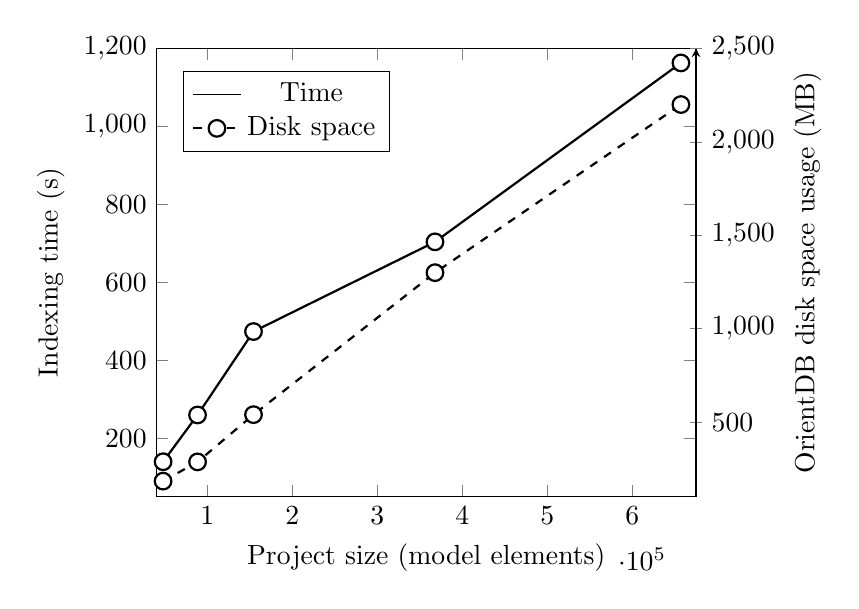
\begin{tikzpicture}
      \begin{axis}[
        xlabel={Project size (model elements)},
        ylabel={Indexing time (s)},
        xmin=40000,xmax=675000,
        ymin=50,ymax=1200
        ]
        \addplot+[black,thick,mark options={solid,mark size=3,fill=white}] coordinates {
          (47891, 140)
          (88451, 260)
          (154281, 474)
          (367840, 704)
          (657228, 1163)
        }; \label{Hplot}
      \end{axis}
      \begin{axis}[
        axis x line=none,
        axis y line=right,
        ylabel={OrientDB disk space usage (MB)},
        xmin=40000,xmax=675000,
        ymin=100,ymax=2500,
        legend style={at={(0.05,0.95)},anchor=north west}
        ]
        \addlegendimage{/pgfplots/refstyle=Hplot}\addlegendentry{Time}
        \addplot+[black,thick,dashed,mark options={solid,mark size=3,fill=white}] coordinates {
          (47891, 184)
          (88451, 287)
          (154281, 540)
          (367840, 1300)
          (657228, 2200)
        }; \addlegendentry{Disk space}
      \end{axis}
    \end{tikzpicture}
  }
  \textbf{Indexing times and index sizes (OrientDB backend)}
\end{center}
